\def\homeworkname{Three networks}
\documentclass[assignment = 1]{homework}

\usepackage{caption, subcaption, pdfpages, float}
\usepackage{graphics, wrapfig, pgf, graphicx}
\usepackage{enumitem}


% pacotes para importar código
\usepackage{caption, booktabs}
\usepackage[section, newfloat]{minted}
\definecolor{sepia}{RGB}{252,246,226}
\setminted{
    bgcolor = sepia,
    style   = pastie,
    frame   = leftline,
    autogobble,
    samepage,
    python3,
    breaklines
}
\setmintedinline{
    bgcolor={}
}

% ambientes de códigos de Python
\newmintedfile[pyinclude]{python3}{}
\newmintinline[pyline]{python3}{}
\newcommand{\pyref}[2]{\href{#1}{\texttt{#2}}}

% \SetupFloatingEnvironment{listing}{name=Código}
% \captionsetup[listing]{position=below,skip=-1pt}

\usepackage{csquotes}
\usepackage[
    style    = verbose-ibid,
    autocite = footnote,
    notetype = foot+end,
    backend  = biber
]{biblatex}
\addbibresource{references.bib}
\usepackage[section]{placeins}

\usepackage[hidelinks]{hyperref}
\usepackage[noabbrev, nameinlink, brazilian]{cleveref}
\hypersetup{
    pdftitle  = {MO412/MC908 - Assignment 1},
    pdfauthor = {Tiago de Paula - 187679}
}

\newcommand{\textref}[2]{
    \hyperref[#2]{#1 \ref*{#2}}
}

\renewcommand{\vec}[1]{\mathbf{#1}}

\DeclareMathOperator{\round}{round}

\usepackage{import, multirow}
\usepackage{tikz}
\usetikzlibrary{matrix}
\usetikzlibrary{positioning}
\usetikzlibrary{automata}
\usetikzlibrary{shapes}

\newenvironment{kmatrix}[1][1.3cm]{
    \begin{tikzpicture}[node distance=0cm]
        \tikzset{square matrix/.style={
                matrix of nodes,
                column sep=-\pgflinewidth, row sep=-\pgflinewidth,
                nodes={draw,
                    minimum height=#1,
                    anchor=center,
                    text width=#1,
                    align=center,
                    inner sep=0pt
                },
            },
            square matrix/.default=#1
        }
}{
    \end{tikzpicture}%
}

\newcommand*{\Scale}[2][4]{\scalebox{#1}{\ensuremath{#2}}}%

\newcommand{\red}[1]{\textcolor{red}{\textbf{#1}}}
\def\qm{?}


\begin{document}
    \pagestyle{main}

    \section{Food Webs}

    \begin{figure}[H]
        \centering
        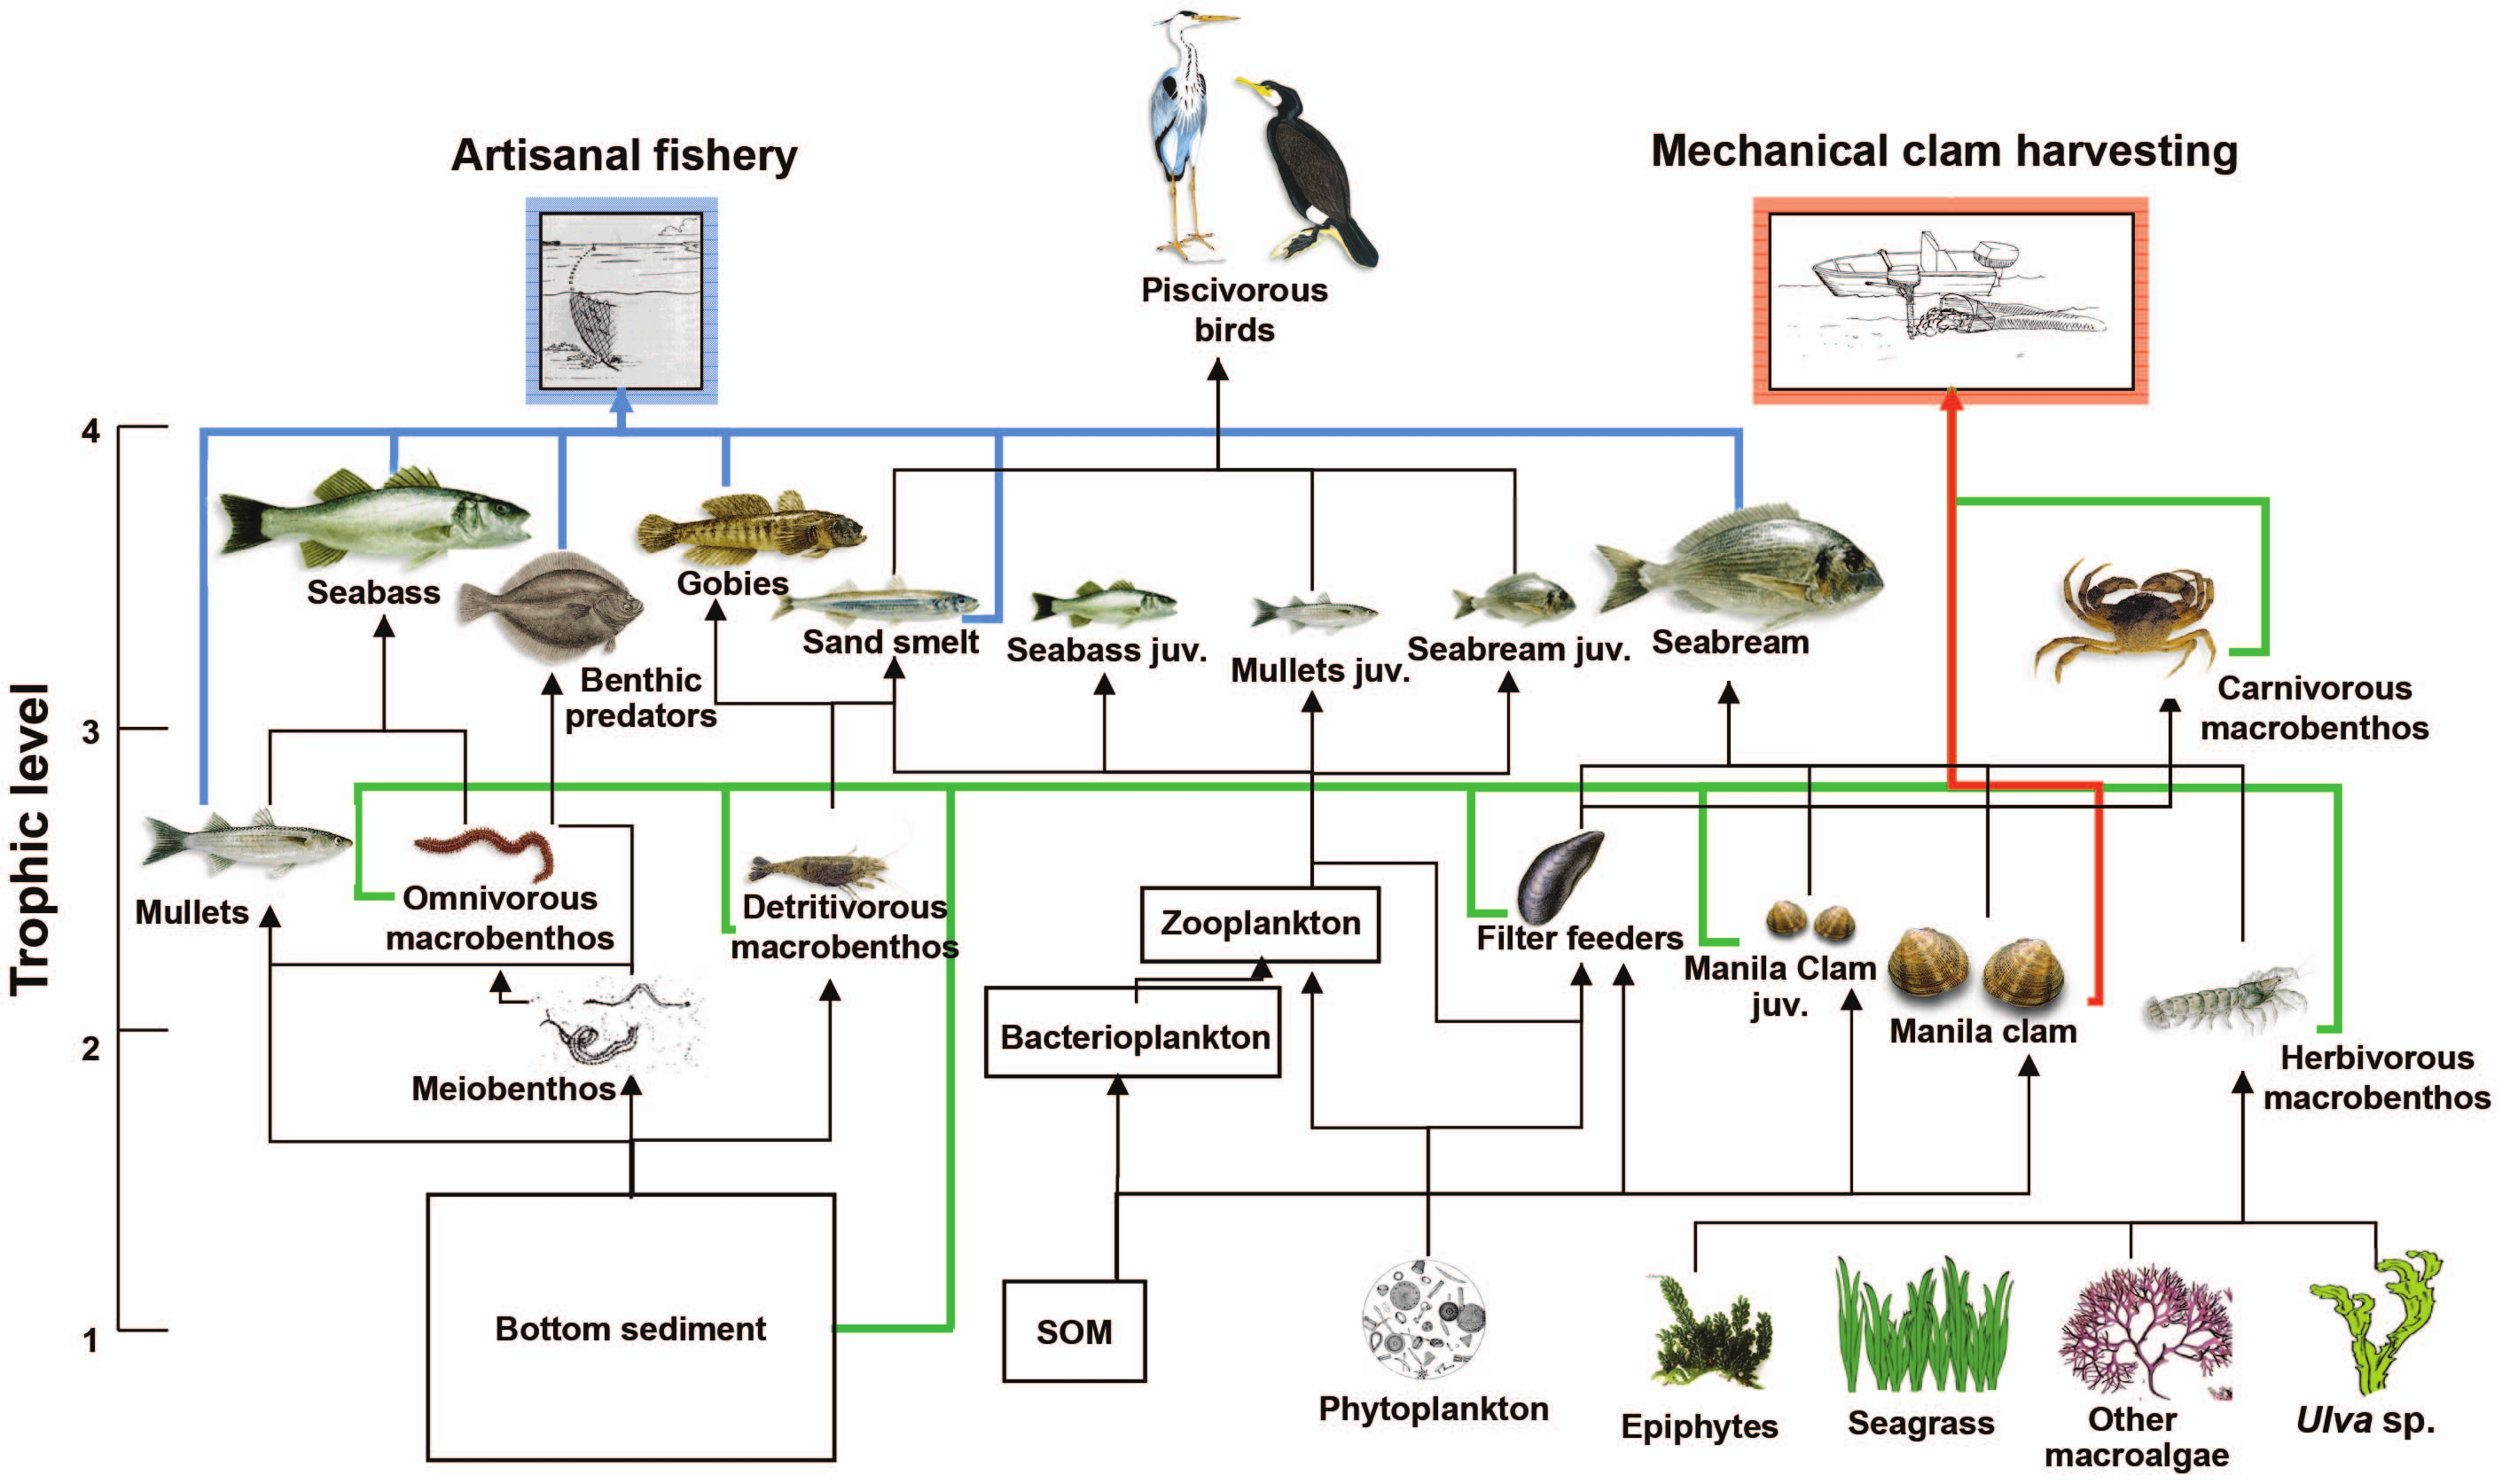
\includegraphics[width=0.9\textwidth]{images/GEN-009.png}

        \caption{Food web diagram of the Venice lagoon. From: \cite{heymans}.}
        \label{fig:food-web}
    \end{figure}

    One of the most common networks used in school comes from biology, the food webs. Here, the nodes usually are species in a given ecological community (Venice lagoon, for \cref{fig:food-web}) and the links map the feeding connection between the species, which species feeds on another.

    \section{Second Network}

    \section{Computer Networks}

    \begin{figure}[H]
        \centering
        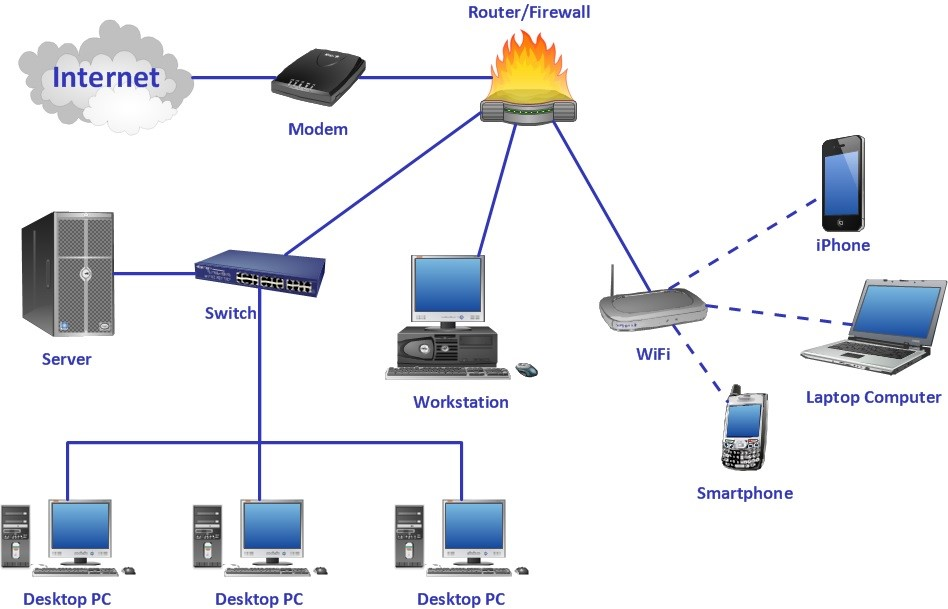
\includegraphics[width=0.7\textwidth]{images/e073f6.jpg}

        \caption{Computer Networking. From: \url{https://www.learnelectronicsindia.com/post/collection-of-computers}.}
        \label{fig:intranet}
    \end{figure}

    Maybe the most famous kind of networks, Computer Networks are composed of computers some other form of hardware communicating between them. The links are either physical cables or some form of wireless communication protocol. These networks are the base of the Internet.

    Different from previous networks, Computer Netorks are physical and can't be fully represented with drawings. However, if you consider some limited aspects of the network, they might still be useful to analyze the topology of a specific netowrk, like \cref{fig:intranet}.

\end{document}
